%%
%% This is file `sample-acmlarge.tex',
%% generated with the docstrip utility.
%%
%% The original source files were:
%%
%% samples.dtx  (with options: `acmlarge')
%% 
%% IMPORTANT NOTICE:
%% 
%% For the copyright see the source file.
%% 
%% Any modified versions of this file must be renamed
%% with new filenames distinct from sample-acmlarge.tex.
%% 
%% For distribution of the original source see the terms
%% for copying and modification in the file samples.dtx.
%% 
%% This generated file may be distributed as long as the
%% original source files, as listed above, are part of the
%% same distribution. (The sources need not necessarily be
%% in the same archive or directory.)
%%
%%
%% Commands for TeXCount
%TC:macro \cite [option:text,text]
%TC:macro \citep [option:text,text]
%TC:macro \citet [option:text,text]
%TC:envir table 0 1
%TC:envir table* 0 1
%TC:envir tabular [ignore] word
%TC:envir displaymath 0 word
%TC:envir math 0 word
%TC:envir comment 0 0
%%
%%
%% The first command in your LaTeX source must be the \documentclass command.
\documentclass[acmtog]{acmart}
\usepackage{listings}
\lstset{language=Go,
  basicstyle=\ttfamily\scriptsize,
  keywordstyle=\color{blue}\ttfamily,
  stringstyle=\color{red}\ttfamily,
  commentstyle=\color{green}\ttfamily}
%%ss[STYLE]{acmart}
%% \BibTeX command to typeset BibTeX logo in the docs
\AtBeginDocument{%
  \providecommand\BibTeX{{%
    \normalfont B\kern-0.5em{\scshape i\kern-0.25em b}\kern-0.8em\TeX}}}

%% Rights management information.  This information is sent to you
%% when you complete the rights form.  These commands have SAMPLE
%% values in them; it is your responsibility as an author to replace
%% the commands and values with those provided to you when you
%% complete the rights form.
\setcopyright{acmcopyright}
\copyrightyear{2022}
\acmYear{2022}
\acmDOI{}


%%
%% These commands are for a JOURNAL article.
\acmJournal{POMACS}
\acmVolume{37}
\acmNumber{4}
\acmArticle{11}
\acmMonth{8}

%%
%% Submission ID.
%% Use this when submitting an article to a sponsored event. You'll
%% receive a unique submission ID from the organizers
%% of the event, and this ID should be used as the parameter to this command.
%%\acmSubmissionID{123-A56-BU3}

%%
%% The majority of ACM publications use numbered citations and
%% references.  The command \citestyle{authoryear} switches to the
%% "author year" style.
%%
%% If you are preparing content for an event
%% sponsored by ACM SIGGRAPH, you must use the "author year" style of
%% citations and references.
%% Uncommenting
%% the next command will enable that style.
%%\citestyle{acmauthoryear}

%%
%% end of the preamble, start of the body of the document source.
\begin{document}

%%
%% The "title" command has an optional parameter,
%% allowing the author to define a "short title" to be used in page headers.
\title{A distributed Filesystem design based on leader worker kuco FS}

%%
%% The "author" command and its associated commands are used to define
%% the authors and their affiliations.
%% Of note is the shared affiliation of the first two authors, and the
%% "authornote" and "authornotemark" commands
%% used to denote shared contribution to the research.
\author{Yiwei Yang}
\email{yangyw@shanghaitech.edu.cn}
\orcid{0000-0001-8011-5868}
\affiliation{
  \institution{ShanghaiTech University}
  \streetaddress{1 R.D. Zhongke}
  \city{Shanghai}
  \state{Shanghai}
  \country{China}
  \postcode{21210}
}

%%
%% By default, the full list of authors will be used in the page
%% headers. Often, this list is too long, and will overlap
%% other information printed in the page headers. This command allows
%% the author to define a more concise list
%% of authors' names for this purpose.
\renewcommand{\shortauthors}{Yiwei Yang}

%%
%% The abstract is a short summary of the work to be presented in the
%% article.
\begin{abstract}
The interaction between the kernel space and the user space is a good offload by sending some of the non confidential IO operation into the user space. The shared worker can scale all the CPU loads to fetch data from the SSDs or Persistent Memory to store them in an unified buffer, once all the scheduled worker finished the operation, the blocked kernel thread will continue to do the operation unique to kernel space permission. This paper will implement the idea and try to scale the operation into a distributed file system that the data is distributed in multi nodes connected with RDMA+PMEM. The writing data will be user space worker distributing data into different nodes and the reading data will be user space worker fetching data from the distributed file system. Since the lock and balance between fetching from the remote nodes can be found to make full use of the bandwidth of NIC and PCIe lane. The scability of the filesystem can be reached.
\end{abstract}

%%
%% The code below is generated by the tool at http://dl.acm.org/ccs.cfm.
%% Please copy and paste the code instead of the example below.
%%
\begin{CCSXML}
  <ccs2012>
  <concept>
  <concept_id>10010520.10010553.10010562</concept_id>
  <concept_desc>Distributed System~Peer to Peer System</concept_desc>
  <concept_significance>500</concept_significance>
  </concept>
  </ccs2012>
\end{CCSXML}

\ccsdesc[500]{LibFS, Distributed FS}

%%
%% Keywords. The author(s) should pick words that accurately describe
%% the work being presented. Separate the keywords with commas.
\keywords{}


%%
%% This command processes the author and affiliation and title
%% information and builds the first part of the formatted document.
\maketitle

\section{Introduction}
As you can also see from the title, this paper is about PM-aware file systems. Currently, after the commercialization of Intel AEP, many teams have started to study the design of applications based on real NVDIMM platforms. The same idea as many previous articles. For example, SplitFS, ZoFS, proposes a hybrid architecture of kernel-state file system and user-state file system collaboration. Since kernel-state file system and user-state file system have their own strengths and weaknesses, it is crucial to enable them to collaborate with each other and take advantage of their strengths. This paper also explores this issue, but at the same time ensures that the architecture has good scalability.

\begin{enumerate}

\item  Currently about PM-aware file systems and other scalability is not good, in the kernel state file system will be limited by VFS, for example in NOVA, when updating files, VFS will put a lock on the upper directory. In user-state file systems, such as in Aerie and Strata, both need to interact with a centralized component, which becomes a bottleneck for scaling.
\item The software overhead is too high for a low-latency memory-level device like PM. For example, kernel-state file systems have system call and VFS call overheads, the
\item There are problems such as stray writes, but PM is persistent and once an error occurs, it is still stored in PM even after reboot.
\end{enumerate}


\section{Proposed approaches}
I would first implement the single thread KucoFS and make the worker node distributed to remote node for file writes and reads. Then I will tune the performance for the worker loads.
\subsection{Overall Overall design}


Adopting Collaborative indexing, which offloads the pathname traversal task to Ulib, encapsulates the relevant information into the request after completion and sends it to Kfs, which directly uses the relevant path addresses to perform metadata adjustment.
\begin{figure}[htbp]
  \centering
  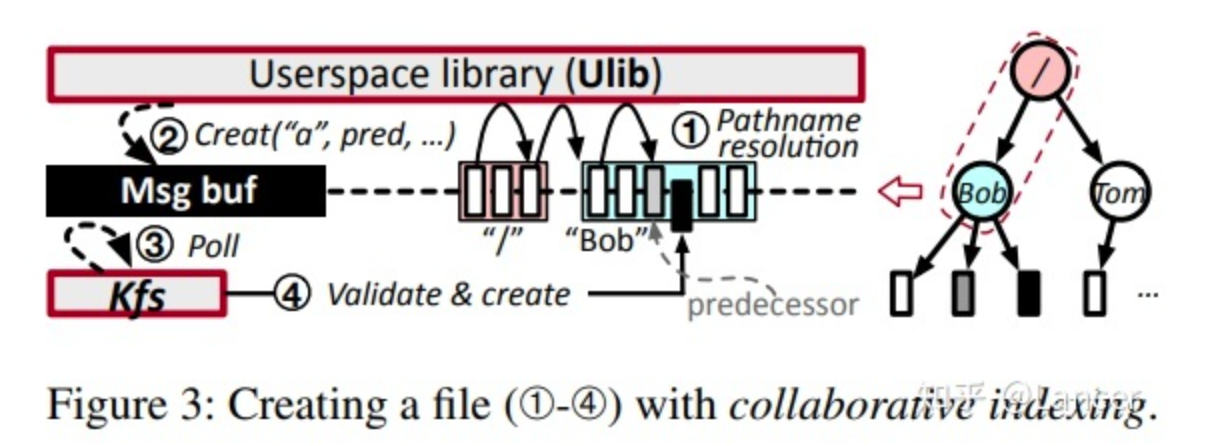
\includegraphics[width=5cm]{./lib.png}
\end{figure}
Two-level locking manages concurrent writes, reducing frequent calls by Kfs during concurrency control and improving scalability; a lease mechanism is used between different processes, and only the process holding the lease can perform write operations. In addition, a userspace range lock is used between different threads of the same process, so that multiple threads can write concurrently to a file.

For data security reasons, such as solving the stray writes problem, the PM space is mapped to the user space in a read-only mode. kuco uses the Three-Phase Write mechanism to implement user space writes in a read-only model (before ulib writes, kfs adjusts the write permissions in the page table, which can be seen due to the interaction between ulib and kfs). (it can be seen that since the interaction between ulib and kfs can become a bottleneck, Kfs uses pre-allocation to allocate more pages for ulib at a time). In addition, Kuco uses the COW method for writing data during write operations.
Due to the COW write method, there will be old and new versions, Kuco uses Versioned Read mechanism to perform read operations in user space, by adding version identification bits in data block mappings, it can guarantee consistent reads without locking, using multiple version mechanism.


\begin{figure}[htbp]
  \centering
  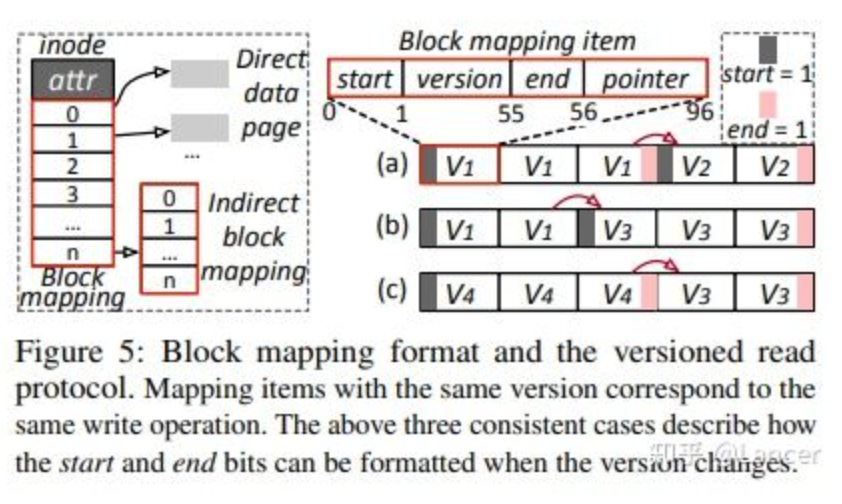
\includegraphics[width=5cm]{./map.png}
  \caption{The mapping between user space and kernel space}
\end{figure}
\subsection{Data Layout}
Data Layout
KucoFS implements a hybrid architecture of DRAM+PM

The inode table is maintained in DRAM, which stores pointers to inodes, where the first pointer in the table points to the root node of the current partition tree, and Ulib finds files in user space based on the inode table. The Block mapping mentioned above is also in DRAM.
The PM is maintained by Operaton log, which guarantees atomic recovery of metadata. There are also data page and metapage, which are managed in 4K.

Crash Consistency and Recovery
Guarantees metadata consistency through strictly ordered updates.
Data pages are updated using the COW mechanism, followed by writing logs to ensure data consistency.
Checkpoint mechanism completes log cleaning operation and instant recovery.

\section{Related work}
The paper called \textit{Gekko FS}, a distributed filesytem that mainly focus on the bandwidth of the read/write. It was to fully utilize the bandwidth of the NIC. Each node have a server daemon and client, and use fast RPC to fetch data to the filesystem. Since the Router can transmit the data from the client to the server with full speed with a good distributor, the scability is linear. Tsinghua University applied the idea of \textit{Gekko FS} and wrote a FS called \textit{MadFS} that top the IO500 board. This bandwidth utilization in their design can be refered to design my user space worker.

The paper published on FAST21, called \textit{Scalable Persistent Memory File System with Kernel-Userspace Collaboration} \cite{chen2021scalable}. This paper presents Kuco, a collaborative user-state and kernel-state file system, with fine-grained task division between the two, minimizing the overhead of the kernel state and providing good scalability.

The UCSC initiated project called \textit{Ceph} which introduced a lot of novel features to the world of distributed filesystems better than \textit{Lustre} and \textit{BeeGFS}, like Consistent Hashing and replication. The backend worker of \textit{Distributed KucoFS} can refer to these designs

\bibliographystyle{ACM-Reference-Format}
\bibliography{perfScope_practical_online_server_performance_bug_inference_in_production_cloud_computing_infrastructures}
\end{document}
\endinput
%%
%% End of file `sample-acmlarge.tex'.
